%%%%%%%%%%%%%%%%%%%%%%%%%%%%%%%%%%%%%%%%%
% University/School Laboratory Report
% LaTeX Template
% Version 3.1 (25/3/14)
%
% This template has been downloaded from:
% http://www.LaTeXTemplates.com
%
% Original author:
% Linux and Unix Users Group at Virginia Tech Wiki 
% (https://vtluug.org/wiki/Example_LaTeX_chem_lab_report)
%
% License:
% CC BY-NC-SA 3.0 (http://creativecommons.org/licenses/by-nc-sa/3.0/)
%
%%%%%%%%%%%%%%%%%%%%%%%%%%%%%%%%%%%%%%%%%

%----------------------------------------------------------------------------------------
%	PACKAGES AND DOCUMENT CONFIGURATIONS
%----------------------------------------------------------------------------------------

\documentclass{article}

\usepackage[version=3]{mhchem} % Package for chemical equation typesetting
\usepackage{siunitx} % Provides the \SI{}{} and \si{} command for typesetting SI units
\usepackage{graphicx} % Required for the inclusion of images
\usepackage{natbib} % Required to change bibliography style to APA
\usepackage{amsmath} % Required for some math elements 
\usepackage[margin=1in]{geometry}
\usepackage{hyperref}
\usepackage[british]{babel}
\selectlanguage{british}


\setlength\parindent{0pt} % Removes all indentation from paragraphs

\renewcommand{\labelenumi}{\alph{enumi}.} % Make numbering in the enumerate environment by letter rather than number (e.g. section 6)

%\usepackage{times} % Uncomment to use the Times New Roman font

%----------------------------------------------------------------------------------------
%	DOCUMENT INFORMATION
%----------------------------------------------------------------------------------------

\title{Computer Vision - Lab 4 \\ Edge Detection and Hough Transform} % Title

\author{Davide Dravindran Pistilli} % Author name

\date{\today} % Date for the report

\begin{document}

\maketitle % Insert the title, author and date

\section{Introduction}
This lab experience focused on detecting a traffic lane and a circular sign. The Canny edge detector was applied along with appropriate Hough transforms for straight line and circle detection.
In order to simplify the detection process, a Gaussian blur was applied to the input image. Though both elements could be correctly detected without any pre-processing, blurring the image allowed to remove most weaker edges with much lower thresholds. After some experimentation, the best option turned out to be a 9x9 kernel with $\sigma=3.5$.

\section{Traffic Lane Detection}
The first step in the traffic lane detection process is the application of the Canny edge detector (\textit{Figure \ref{img_canny}}). The two thresholds are set to $118$ and $129$, respectively, but they can be changed quite significantly while still obtaining the same end result.

\begin{figure}[h]
\begin{center}
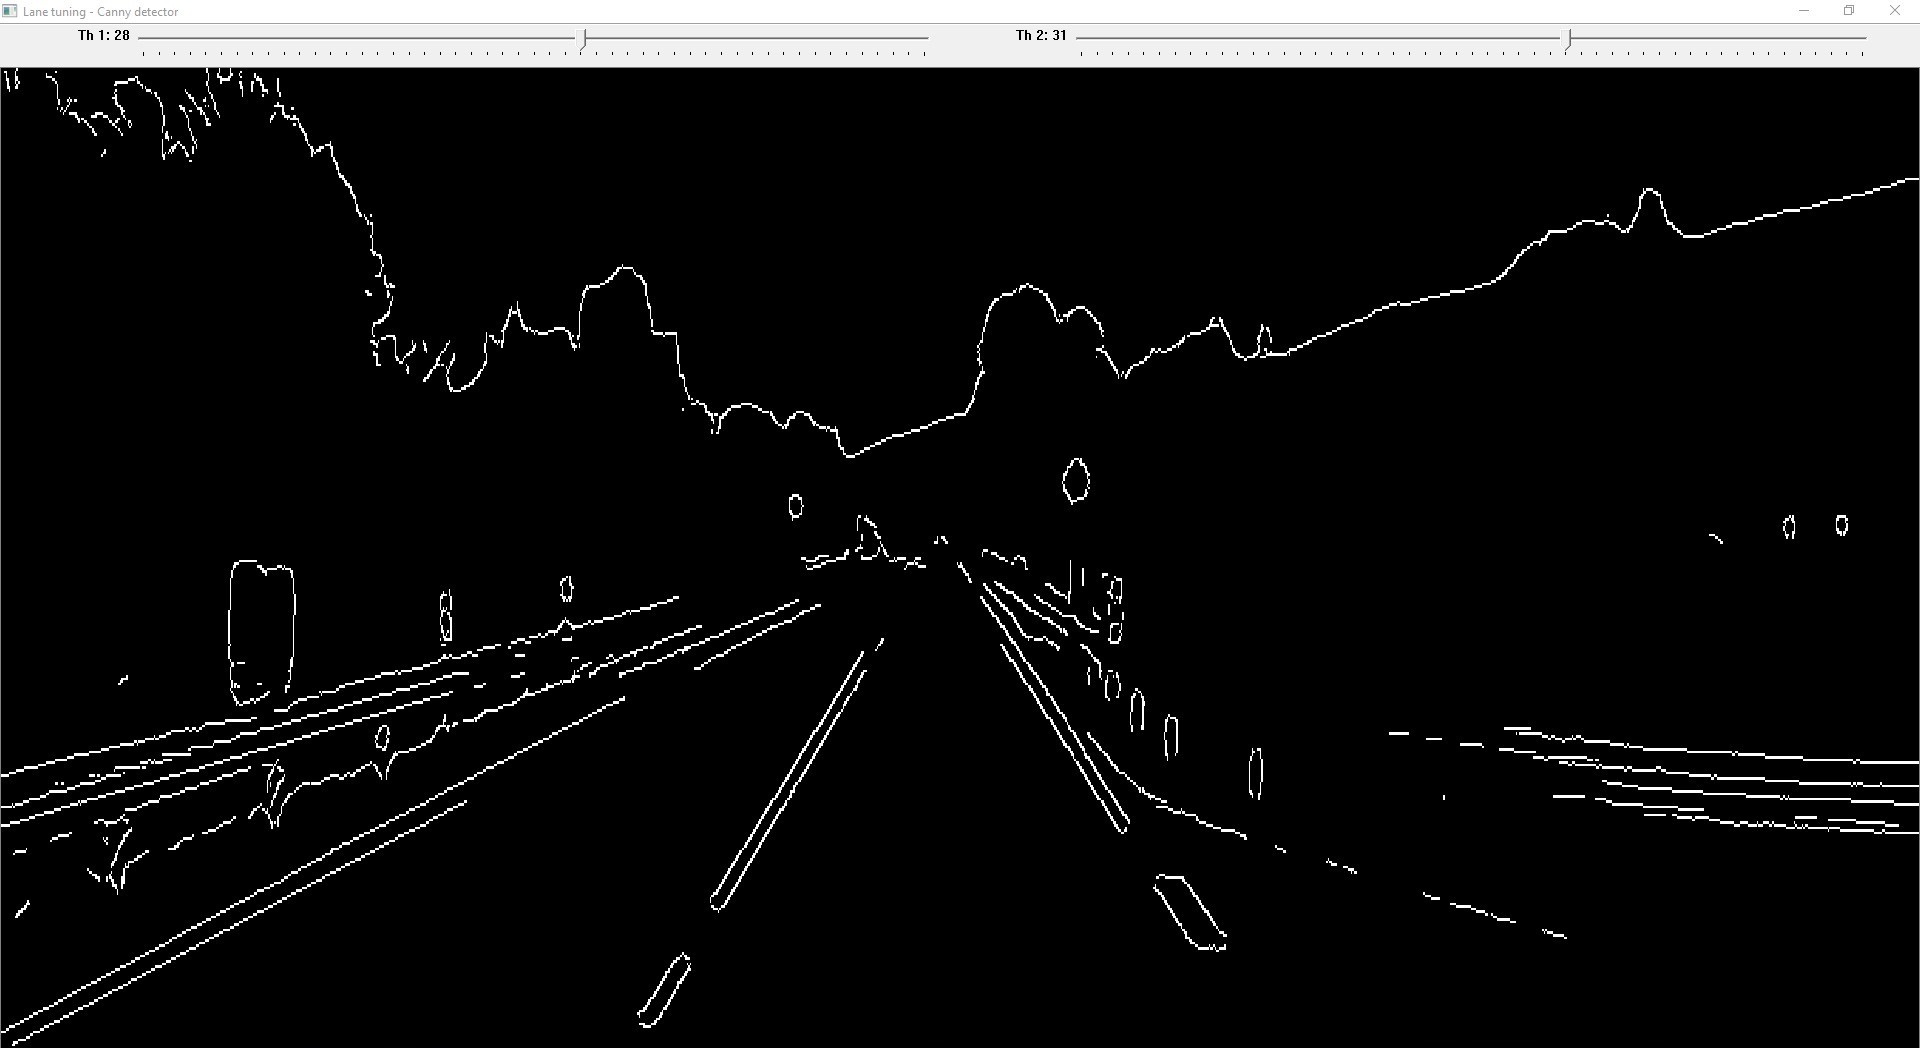
\includegraphics[width=1\textwidth]{images/canny}
\caption{\footnotesize{Canny edge detector.}}
\label{img_canny}
\end{center}
\end{figure}

Canny's output is then passed to the Hough transform used to find straight lines (\textit{Figure \ref{img_hough_lines}}). No pre-processing is strictly required. However, by introducing a slight horizontal dilation (1x3 structuring element) it becomes easier to tune Hough's parameters in order to correctly detect the right traffic lane. The three tuned parameters are set as follows:
\begin{itemize}
\item \textbf{Distance Resolution}: $1.0$;
\item \textbf{Angular Resolution}: $0.388$ (a bit more than $\pi/10$);
\item \textbf{Accumulator Threshold}: $139$.
\end{itemize} 
Slight variations in distance resolution and accumulator threshold result in the same output. Angular resolution, however, has to remain close to the chosen value. Indeed, an excessive variation leads to the detection of other lines that have higher accumulator values than the required ones.

\begin{figure}[h]
\begin{center}
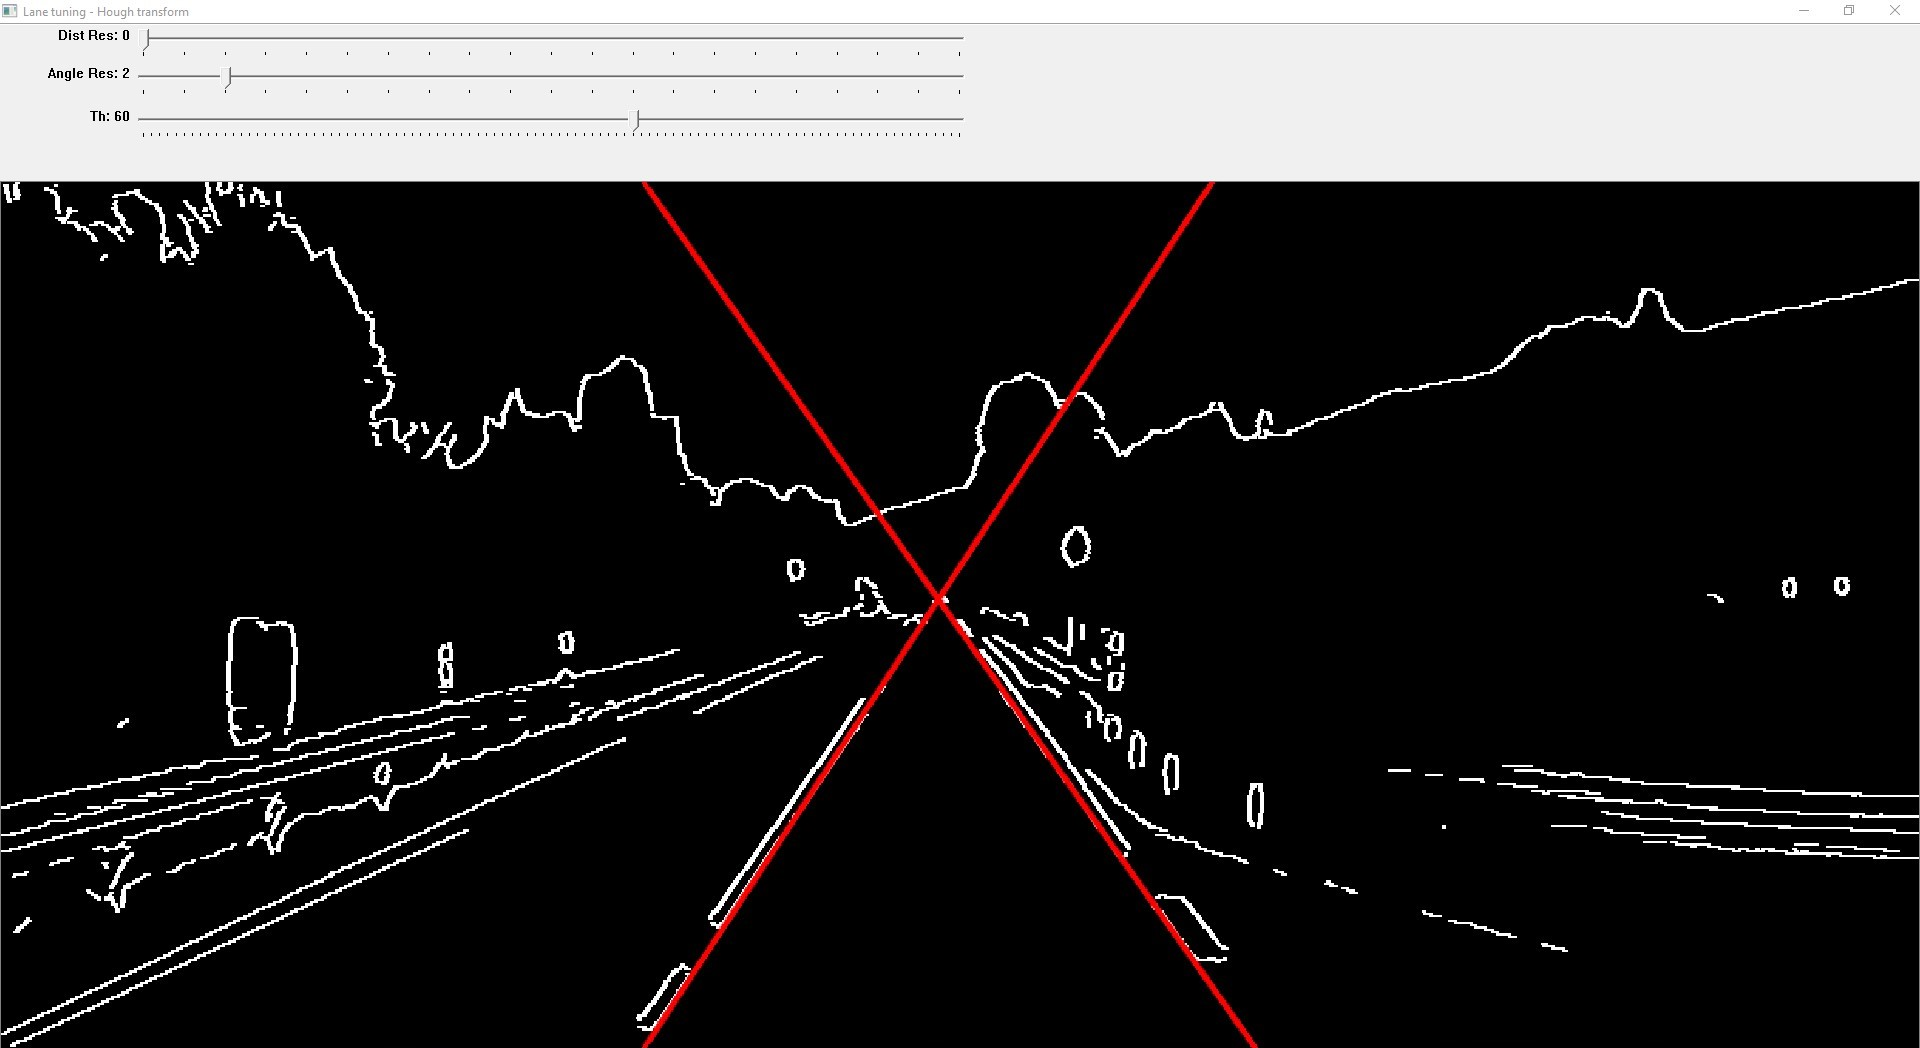
\includegraphics[width=1\textwidth]{images/hough_lines}
\caption{\footnotesize{Hough transform for line detection.}}
\label{img_hough_lines}
\end{center}
\end{figure}

\section{Sign Detection}
Sign detection is performed through the OpenCV function \texttt{cv::HoughCircles}. This function already includes the Canny edge detector, so it need not be applied separately, which was, instead, done for the traffic lane detection phase.
The result is quite precise (\textit{Figure \ref{img_hough_circles}}), but parameter tuning is more difficult than with traffic lane detection. The result, in fact, is quite sensitive to any parameter changes and, since both the Canny detector and the Hough transform are performed at the same time, there is no way to visualise the intermediate Canny output. Furthermore, circle detection takes longer than line detection, especially with low thresholds and minimum distance between centres.
The final parameters are:
\begin{itemize}
\item \textbf{Resolution}: $1.0$;
\item \textbf{Minimum Distance}: $1.0$;
\item \textbf{Threshold 1}: $13.92$;
\item \textbf{Threshold 2}: $18.63$;
\item \textbf{Minimum Radius}: $1$;
\item \textbf{Maximum Radius}: $4$.
\end{itemize}

\begin{figure}[h]
\begin{center}
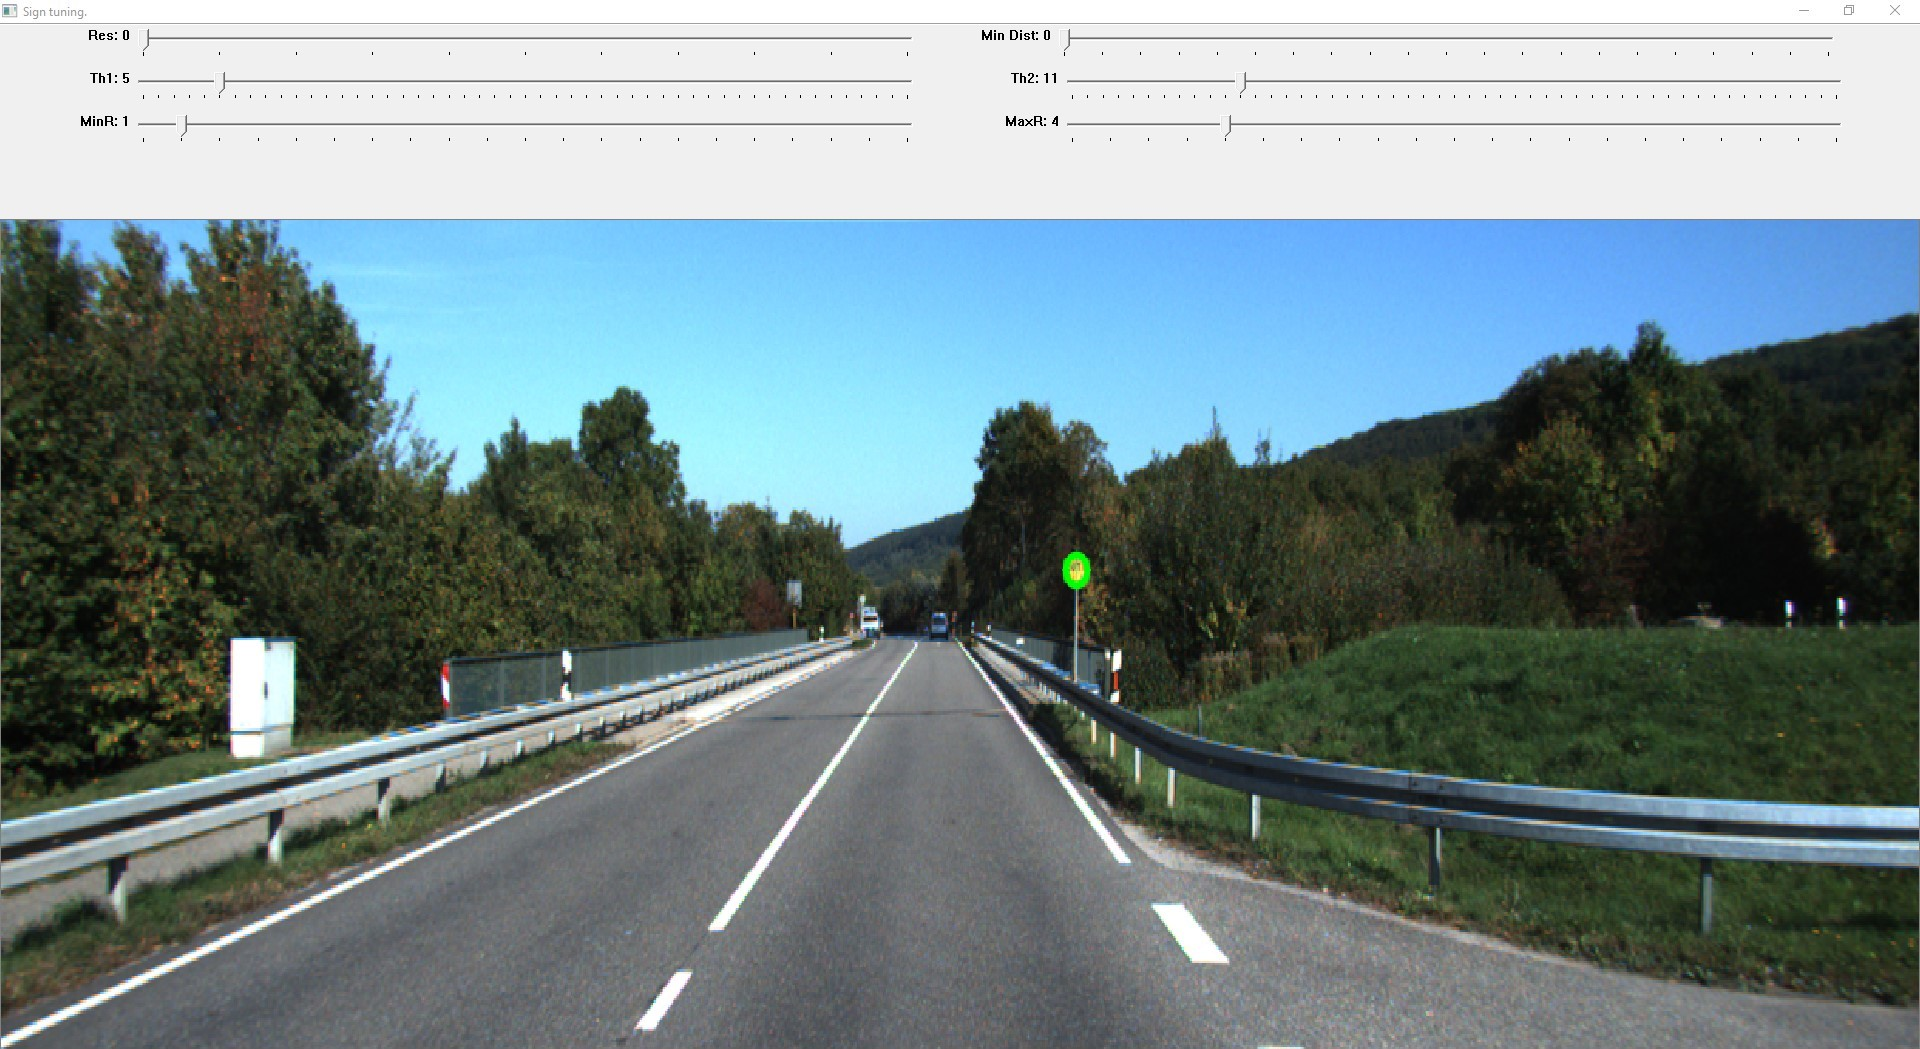
\includegraphics[width=1\textwidth]{images/hough_circles}
\caption{\footnotesize{Hough transform for circle detection.}}
\label{img_hough_circles}
\end{center}
\end{figure}

\section{Result}
The overall result is displayed in \textit{Figure \ref{img_result}}.

\begin{figure}[h]
\begin{center}
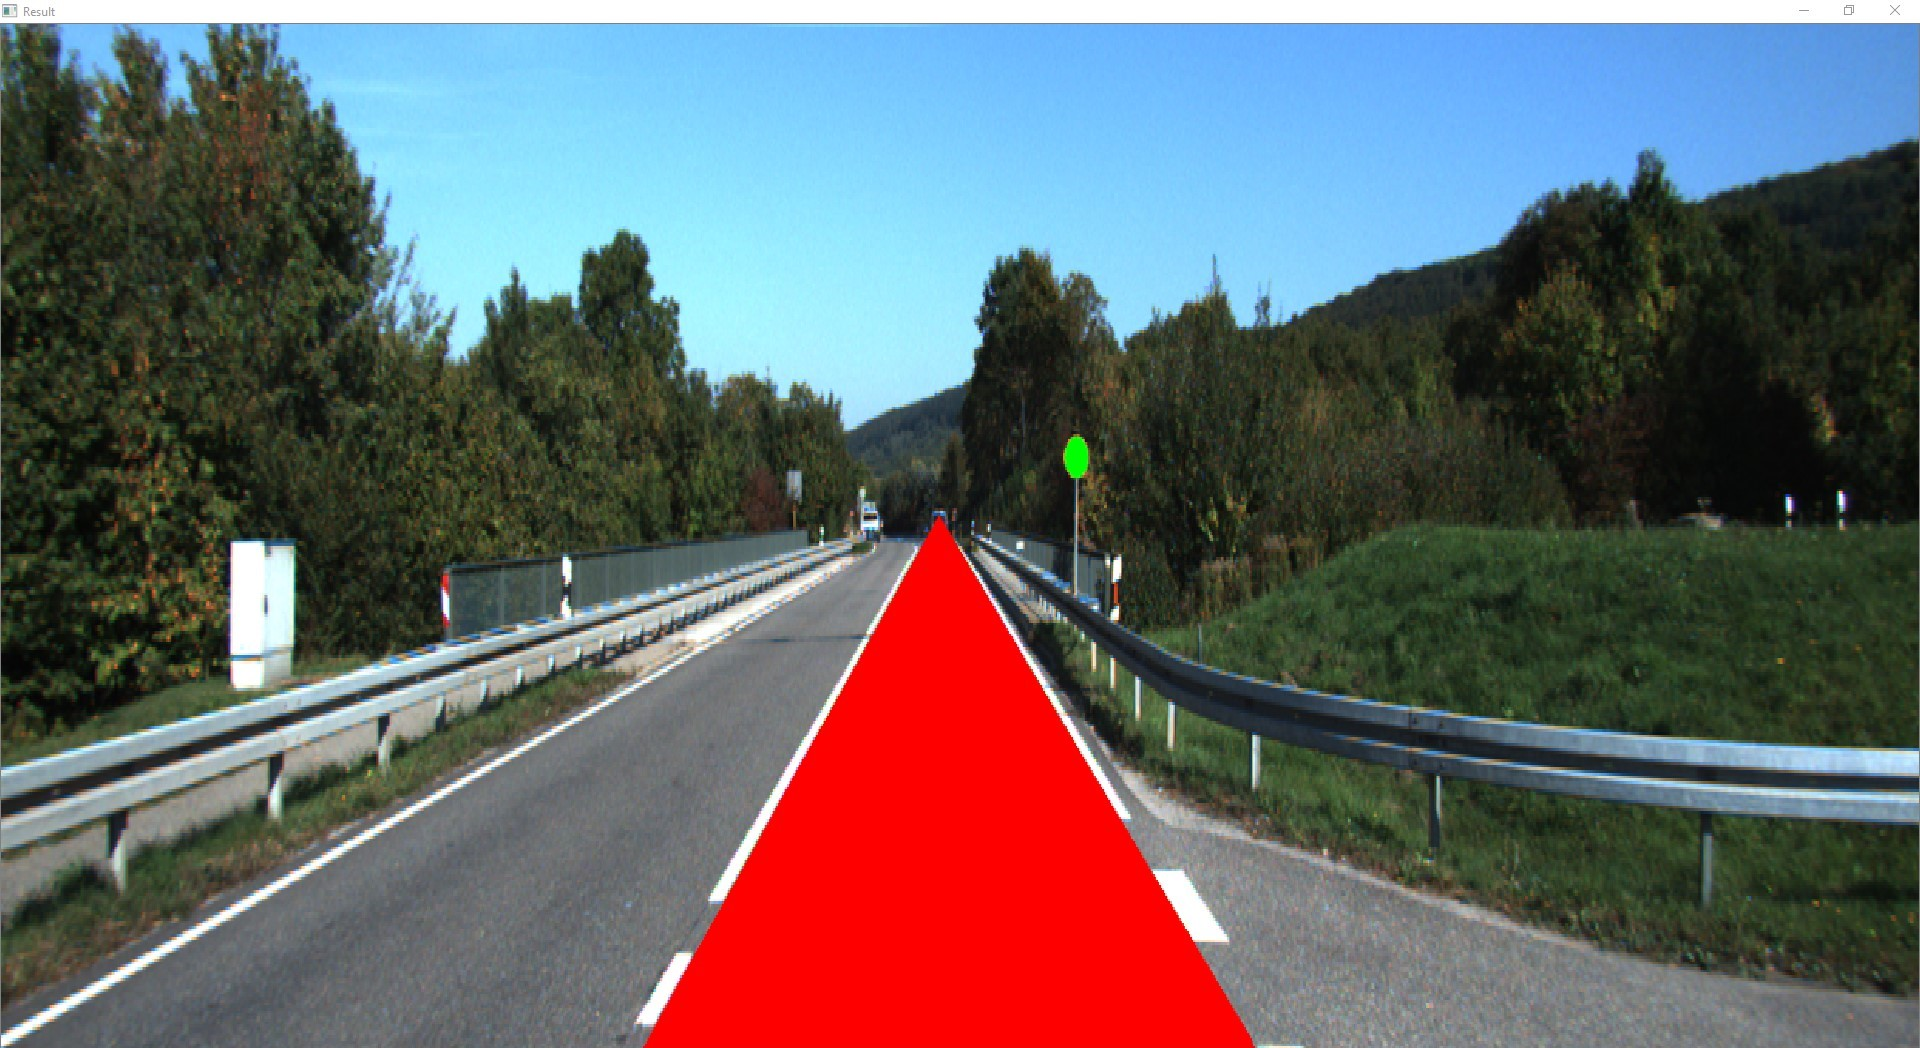
\includegraphics[width=1\textwidth]{images/result}
\caption{\footnotesize{Overall result.}}
\label{img_result}
\end{center}
\end{figure}

\end{document}